\chapter{Project Logic Diagrams}


\section{Work Flow Diagram}
 In order to achieve effective project planning, three workflow diagrams are made: for the baseline, mid-term and final review, respectively. In all these diagrams, colours are used to identify work packages. The lightness of the colours signifies the order of work-packages, the lightest groups having to be completed before the darker groups.

\subsection*{Baseline Review Workflow Diagram}
The final deliverables of the baseline report are going to be the few most feasible configurations of the aircraft.
Taking as input the main user requirements from \autoref{tab:user_requirements}, the risk analysis and the functional analysis can be performed in parallel, especially since the former mainly concerns organisational risks at this stage of the project. The main outcome of the risk analysis is the risk map, showing the probability and severity of the most important risks. 

Simultaneously, the functional analysis process results in the functional breakdown and the functional flow diagram, both of which are required for the requirement analysis and the latter also for the allocation of resources. The process of allocating resources also takes the risk map into account, and results in the organogram, Gantt chart, workflow diagram (this diagram) and work breakdown structure. Moreover, the functional analysis also involved the market analysis, resulting in the profit analysis and the summary of discussion with stakeholders. Together with the list of sustainability objectives, these are the prerequisites for performing the requirement analysis.

Furthermore, the requirement analysis is performed using the requirement discovery tree, and ending with the preliminary list of technical requirements. Afterwards, option generation is performed by means of making the option discovery tree. Then, the clearly unfeasible options are discarded, ending with a list of 20-30 possible aircraft configurations. Finally, a simple trade-off procedure is performed between the remaining options. That results in the 2-3 most feasible configurations.

\begin{figure}[H]
    \centering
    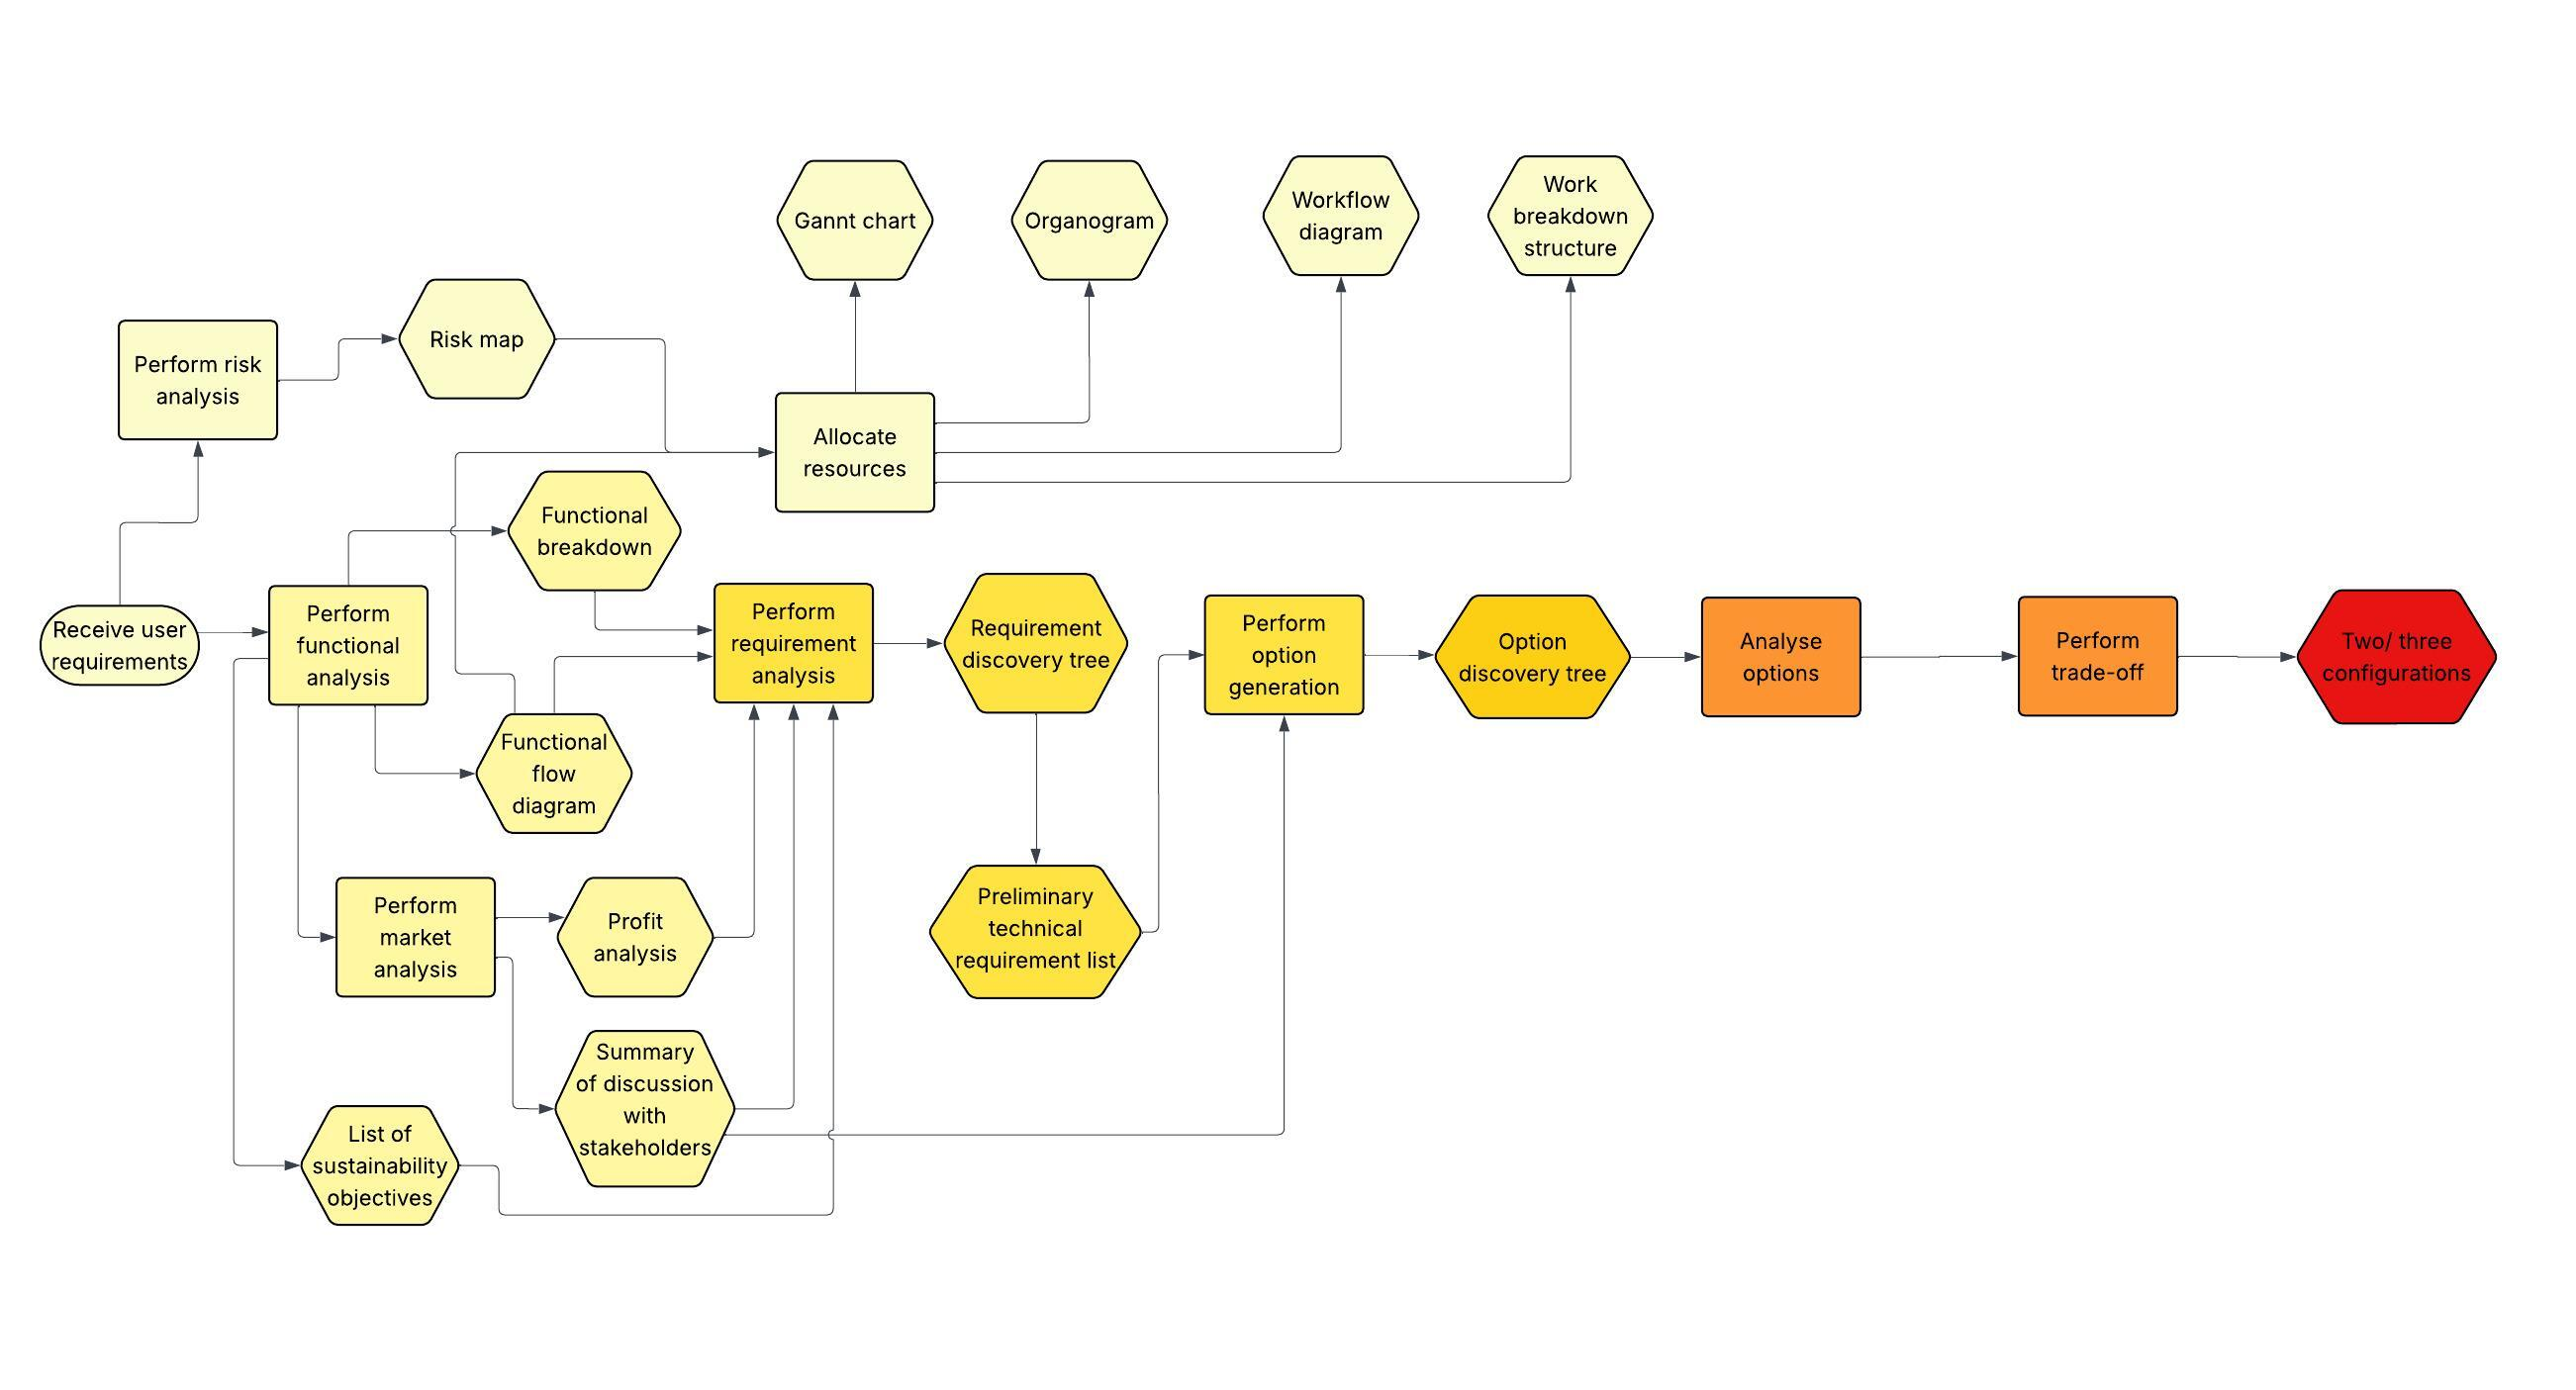
\includegraphics[width=1.4\linewidth, angle=90]{figures/Baseline_workflow.jpeg}
    \caption{Baseline Review Workflow Diagram}
    \label{fig:workflow_baseline}
\end{figure}

\subsection*{Midterm Review Workflow Diagram}

The Midterm Review mostly concerns itself with the preparation and execution of the trade-off between the design options shortlisted in the baseline review. This dictates the focus of the workflow diagram presented in \autoref{fig:workflow_midterm}. The trade off can be split into formally formulating the trade-off criteria and carrying out preliminary weight,  aerodynamic and life cycle analysis to the extent needed to evaluate the options against the criteria. To determine that extent, it is advisable to formulate the criteria first, and conduct the analysis later, although there are no direct input-output lines between the two.

For the trade-off criteria, the degree of versatility will be the primary factor. It will be balanced by additional performance (lower weight, higher endurance, etc.), the ease of manufacturing, as well as logistical/organizational and sustainability aspects of the designs.

\begin{figure}[H]
    \centering
    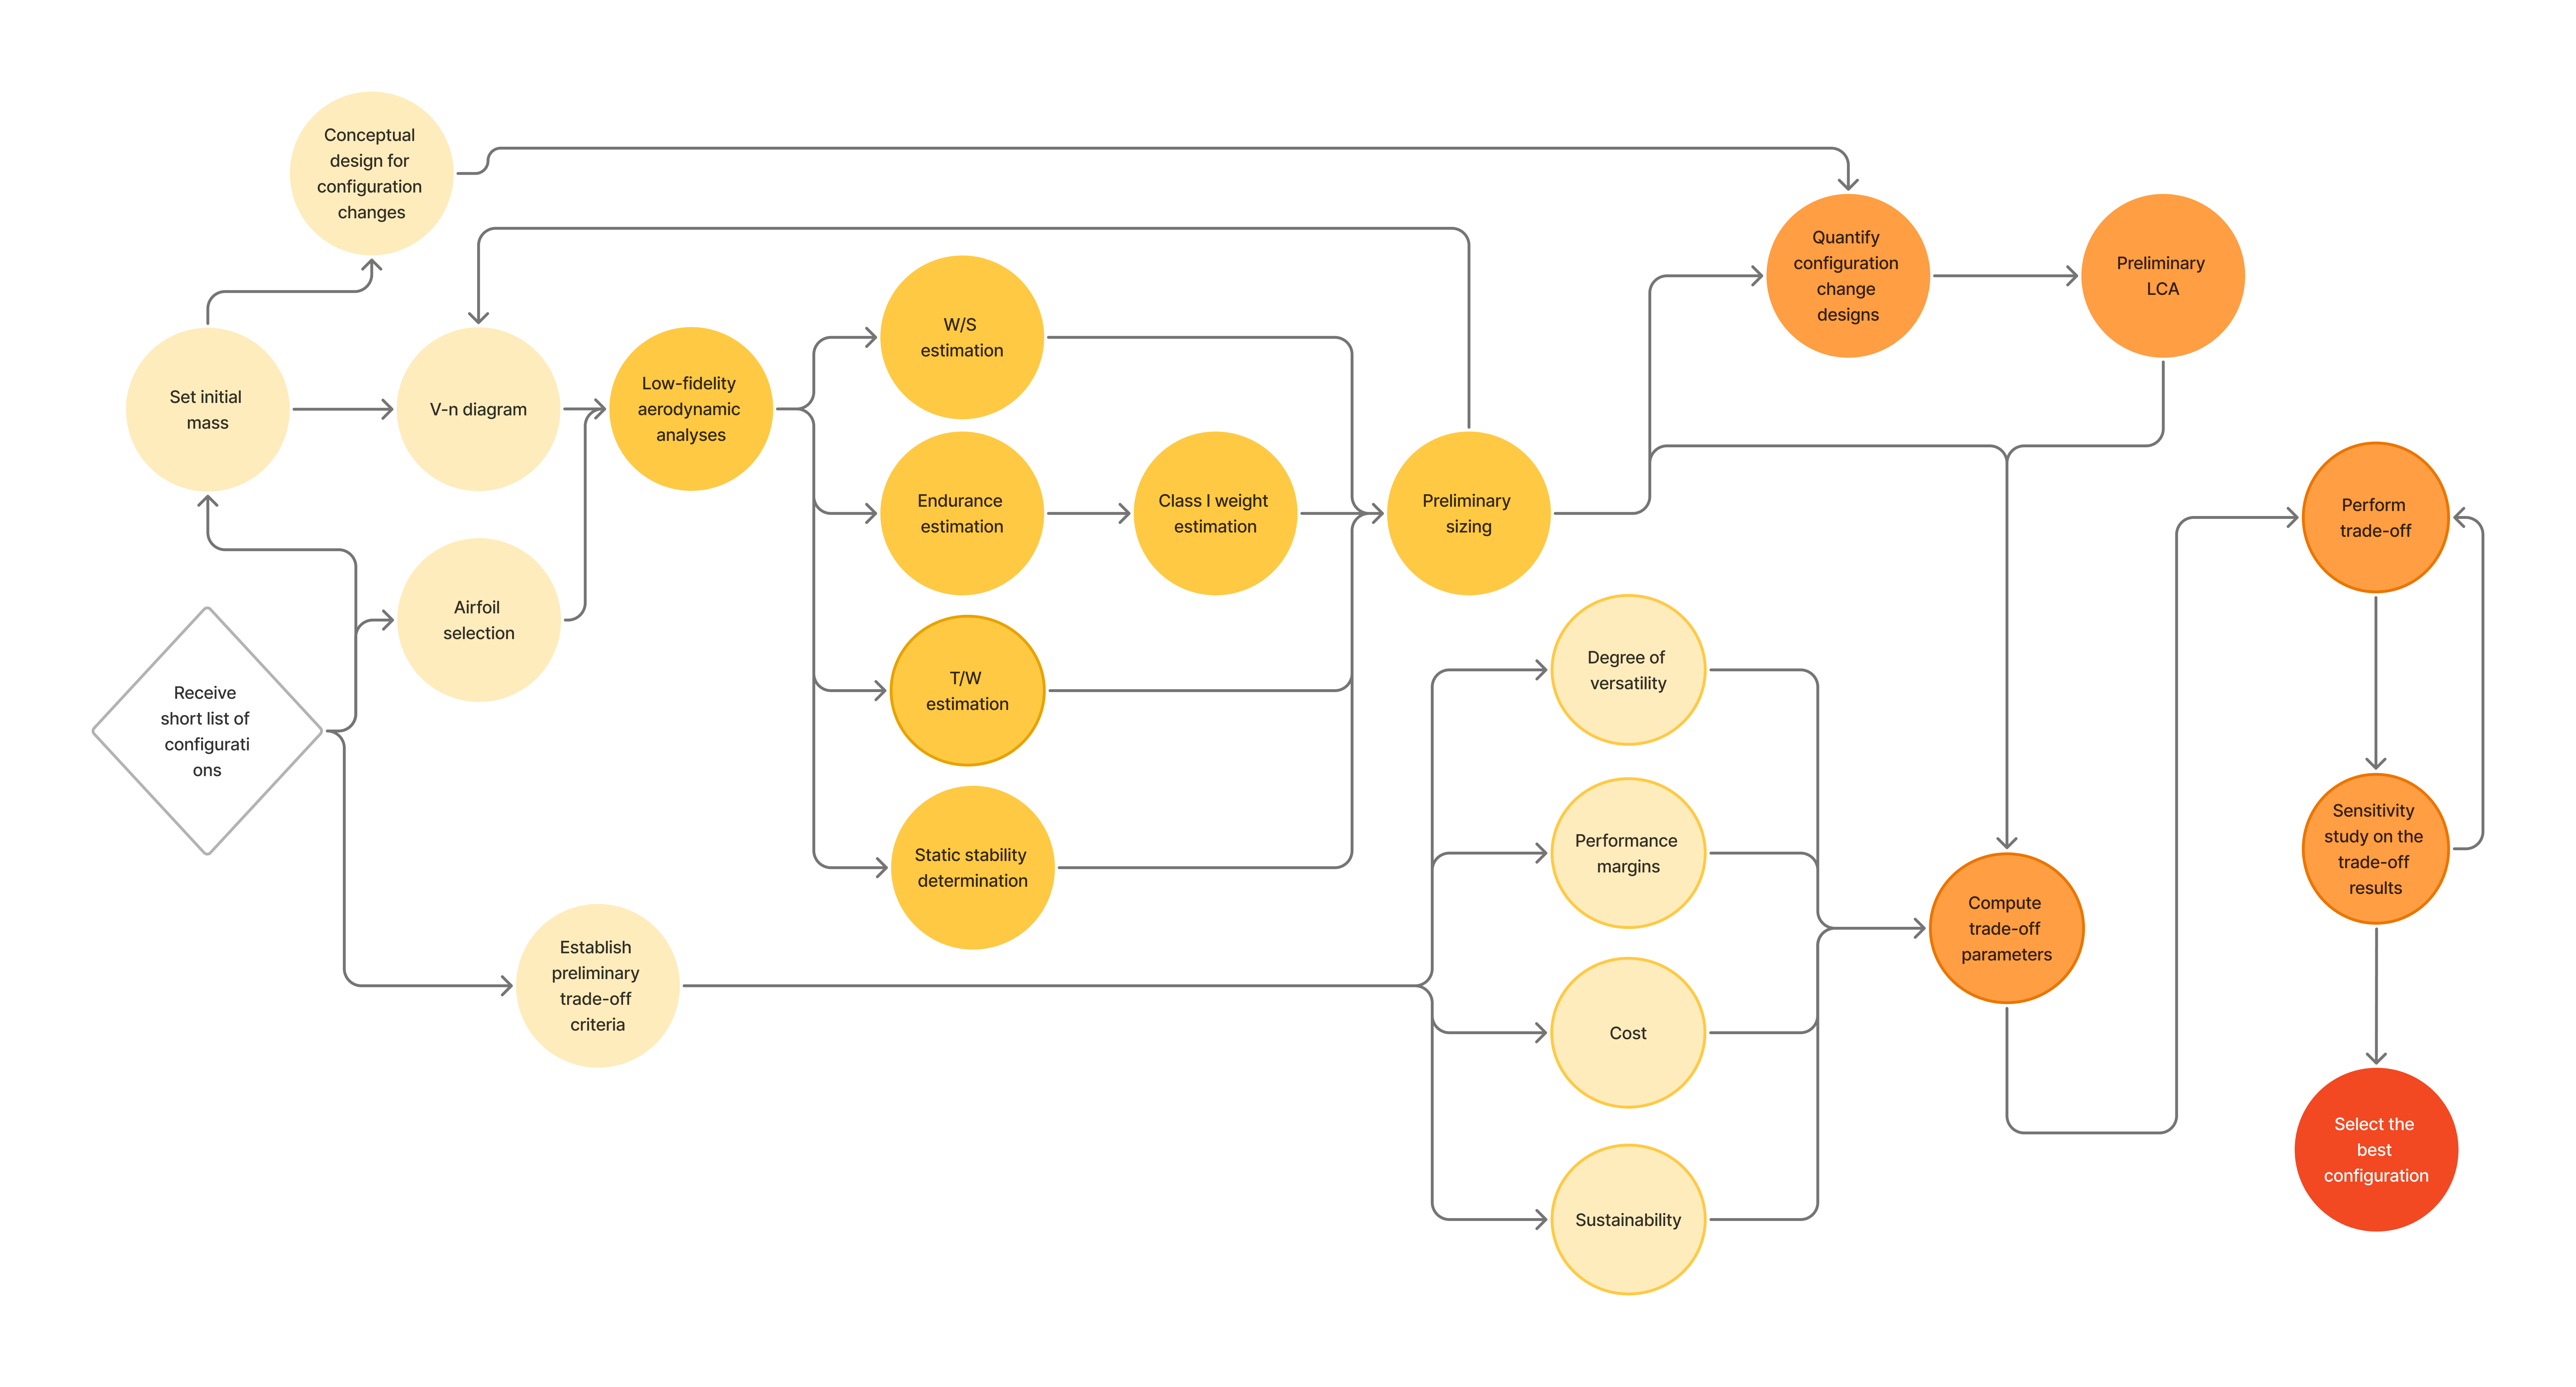
\includegraphics[width=1.4\linewidth, angle=90]{figures/Mid-term workflow.jpg}
    \caption{Mid-term Review Workflow Diagram}
    \label{fig:workflow_midterm}
\end{figure}

\newpage

\subsection*{Final Review Workflow Diagram}

The first work package within the final stage of the project is initiated with the received proposal of the best design concept from the mid-term review. Then, system requirements are used as the starting point for further steps. In parallel, the focus of the design is established and the wing planform parameters are defined. The latter includes the computation of the required lift force, finding the required size of the lifting surfaces (wings) and defining the wing planform parameters, such as the sweep and dihedral angle and the taper ratio. 

At this point, the main subsystems can be designed, such as the wing (more detailed) and fuselage geometry, wing box architecture, tail geometry and position (if applicable), main control surface geometry, aircraft material, connections between the subsystems, engine integration architecture, and fuel storage specifications. Subsequently, the aircraft flight dynamics, aerodynamic and structural models are created, verified and validated, followed by creating the performance summary. From the performance summary, there is a feedback loop where the performance is compared with system requirements and wing parameters are modified accordingly.

In the next work package, the aforementioned models are used to create, verify, validate and perform flutter and fatigue analyses, after which there are again feedback loops in which the flutter speed and fatigue performance are compared with their corresponding requirements. In parallel to these analyses, the design of the main control system is initiated.

Subsequently, the sensor and actuator positioning and characteristics are defined, upon which the main control system performance is evaluated, the control parameters are tuned, and the main control system is modified accordingly. Simultaneously, the main structure is integrated with the payload. Finally, the manufacturing plan is devised, followed by the final sustainability evaluation, while in parallel the operations plan is set up. Both branches contribute to the final product specification.

% \begin{figure}[H]
%     \centering
%     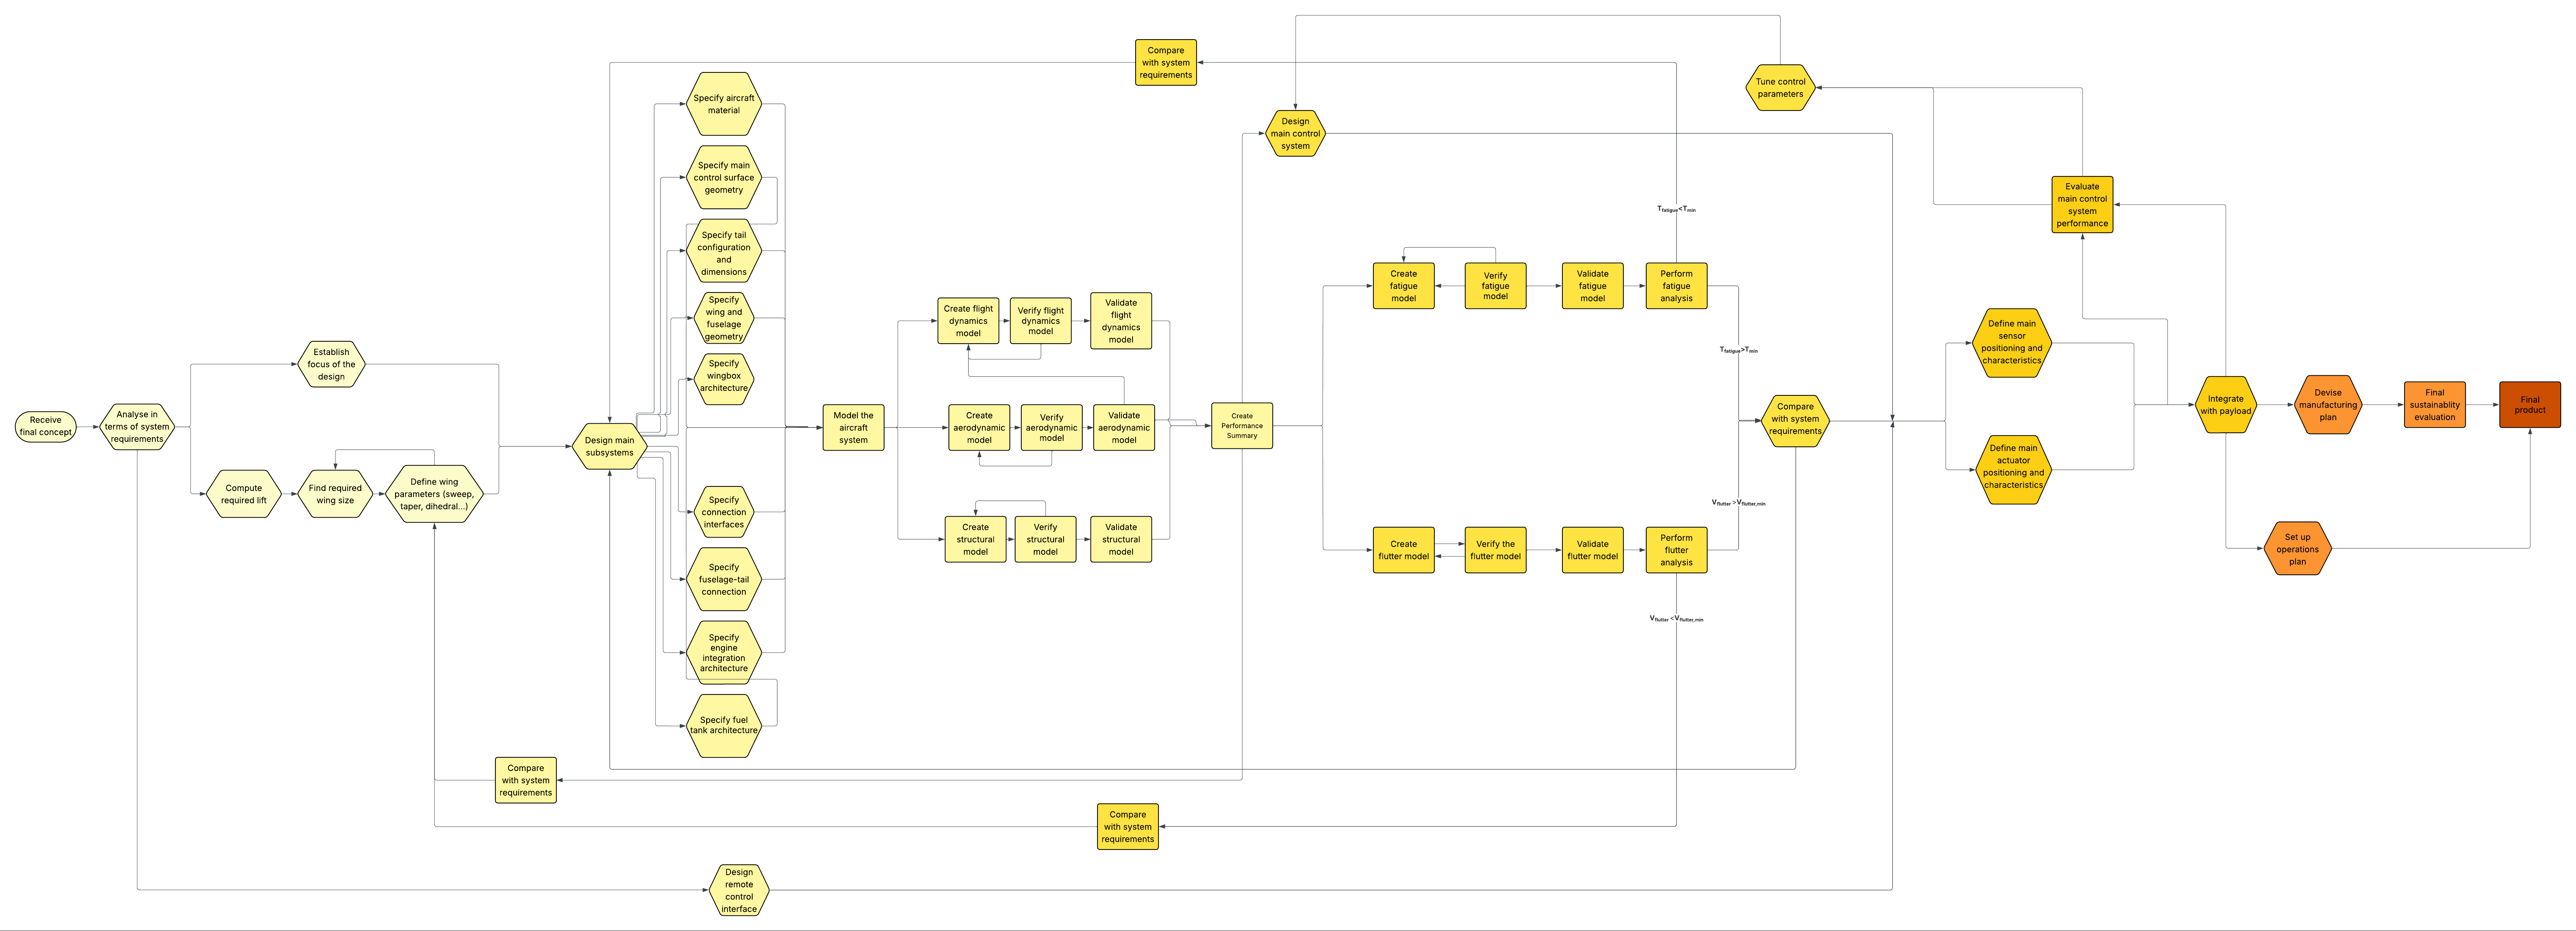
\includegraphics[width=1.4\linewidth, angle=90]{figures/Final workflow.png}
%     \caption{Final Review Workflow Diagram}
%     \label{fig:workflow_final}
% \end{figure}
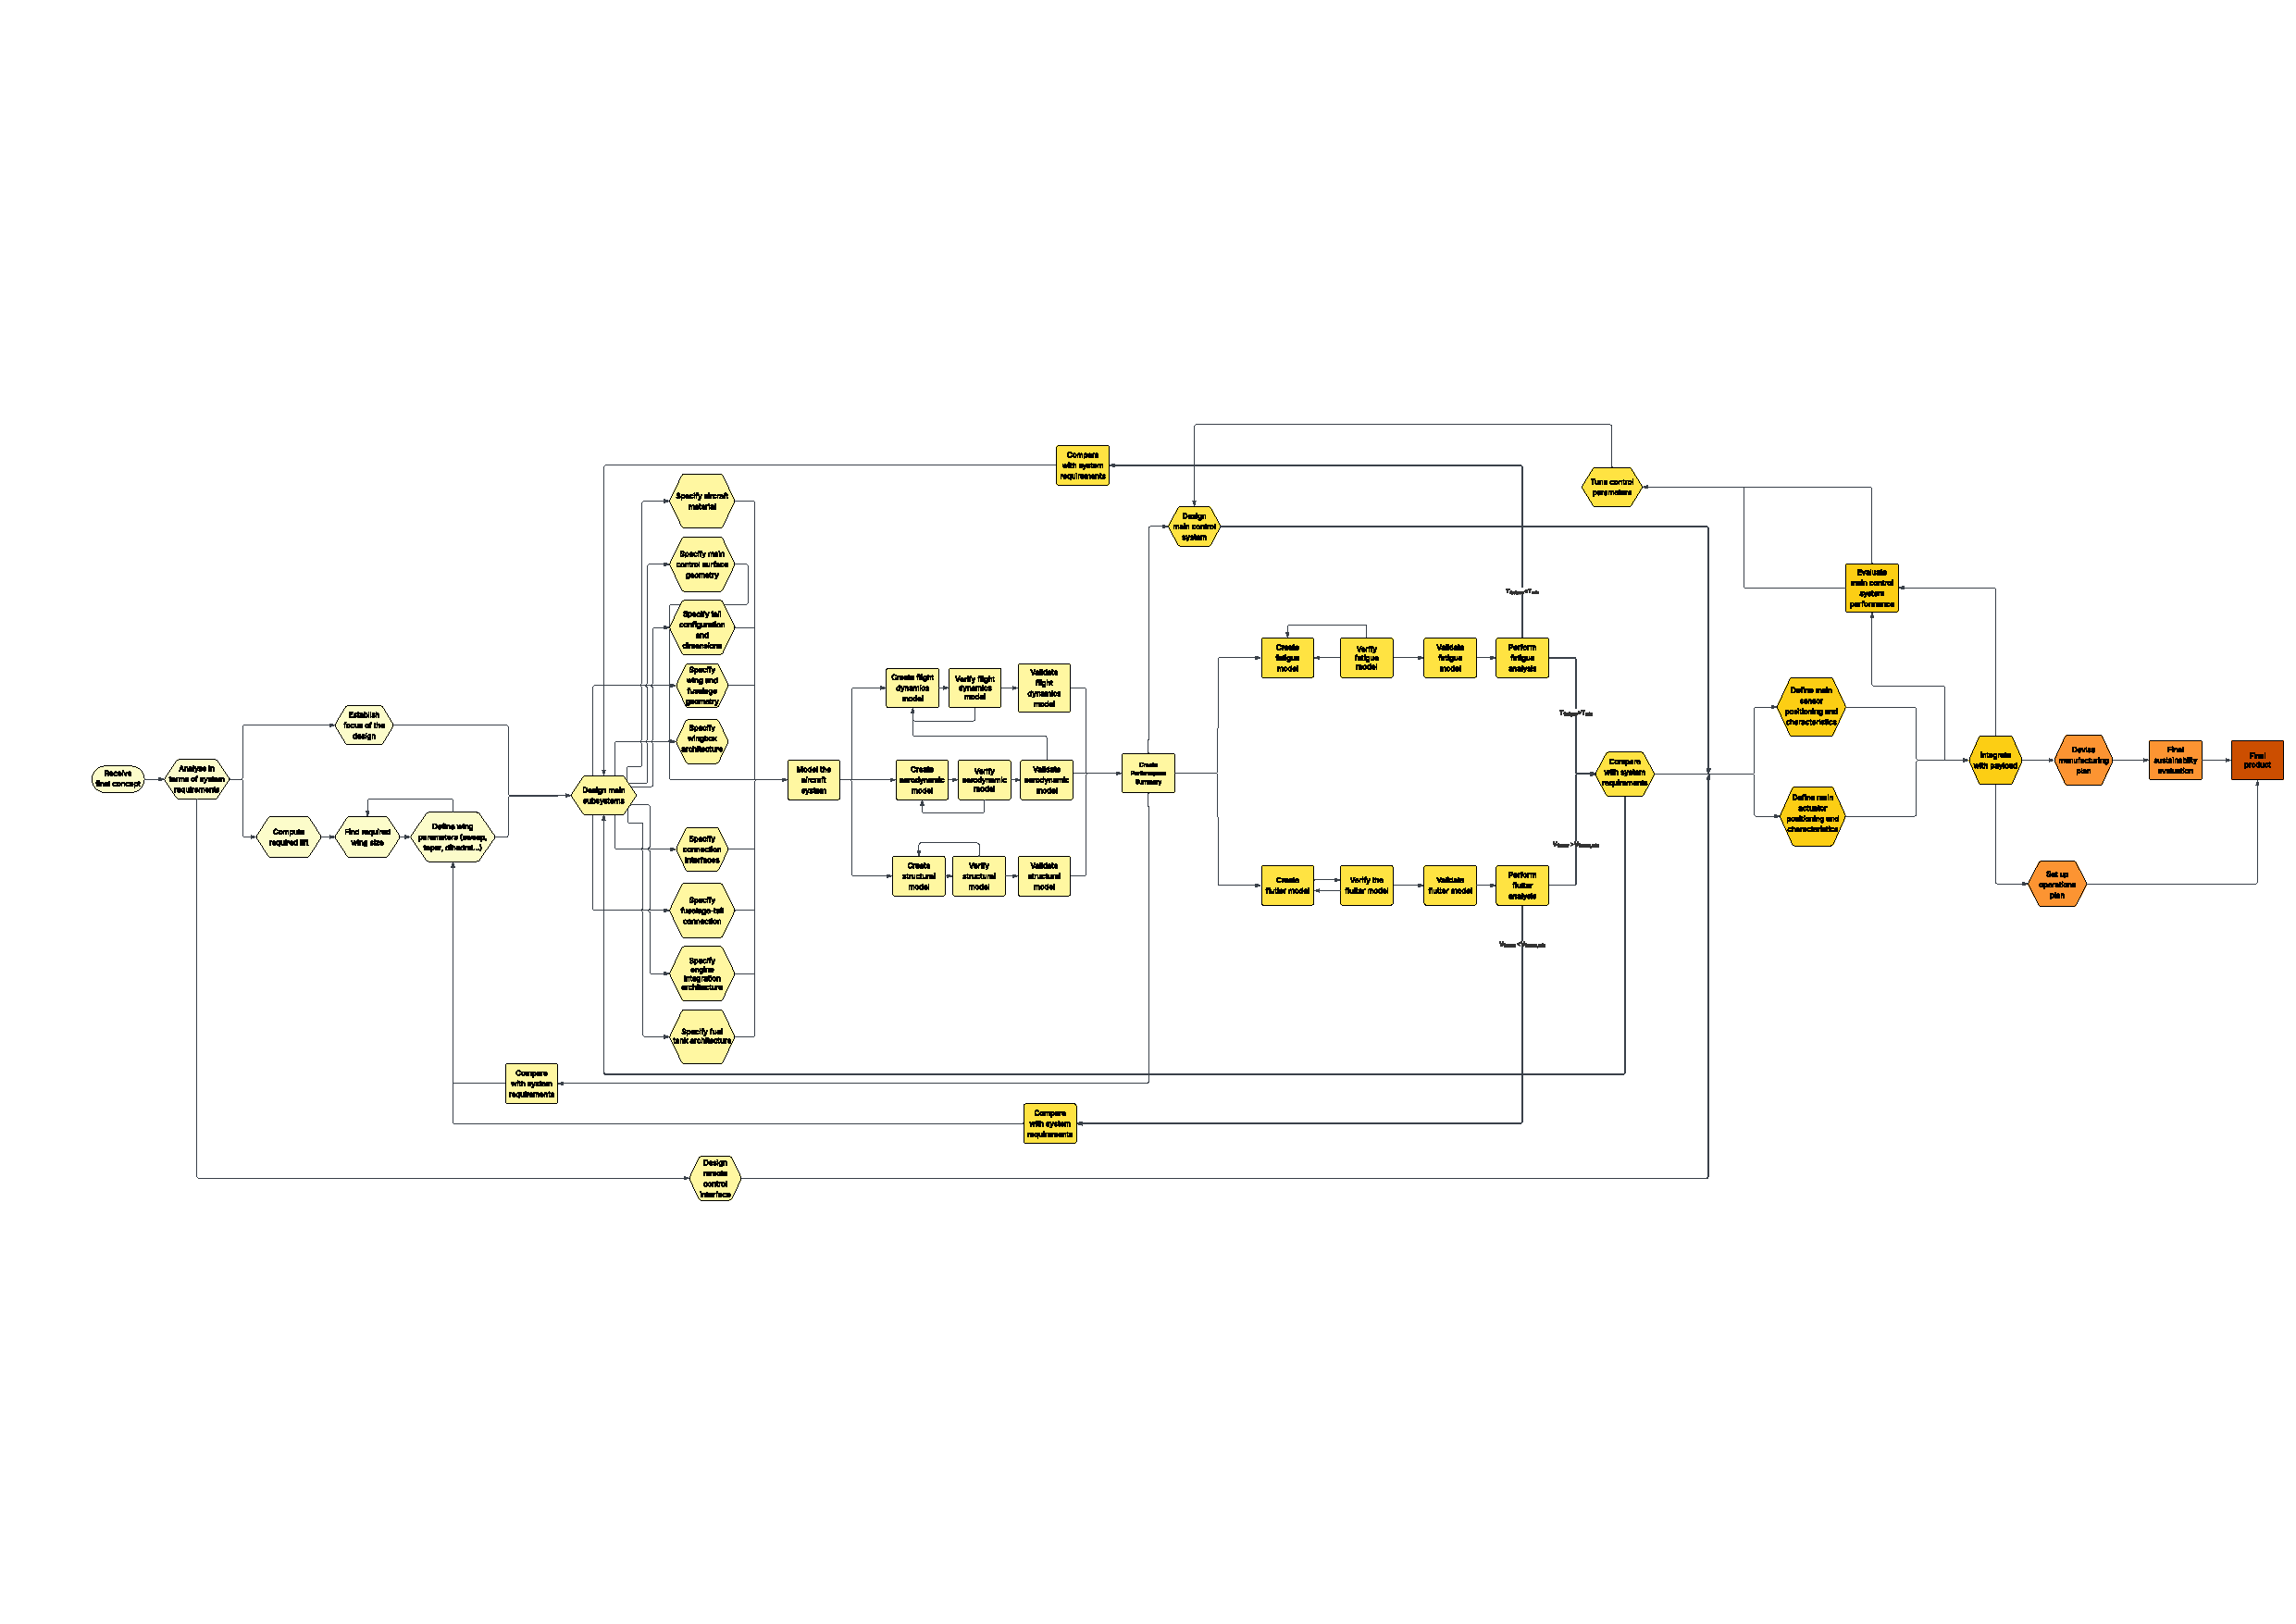
\includepdf[pages=-,fitpaper=true, width=420mm, keepaspectratio]{figures/Work-flow diagram (1).pdf}

% \begin{figure}[H]
%     \centering
%     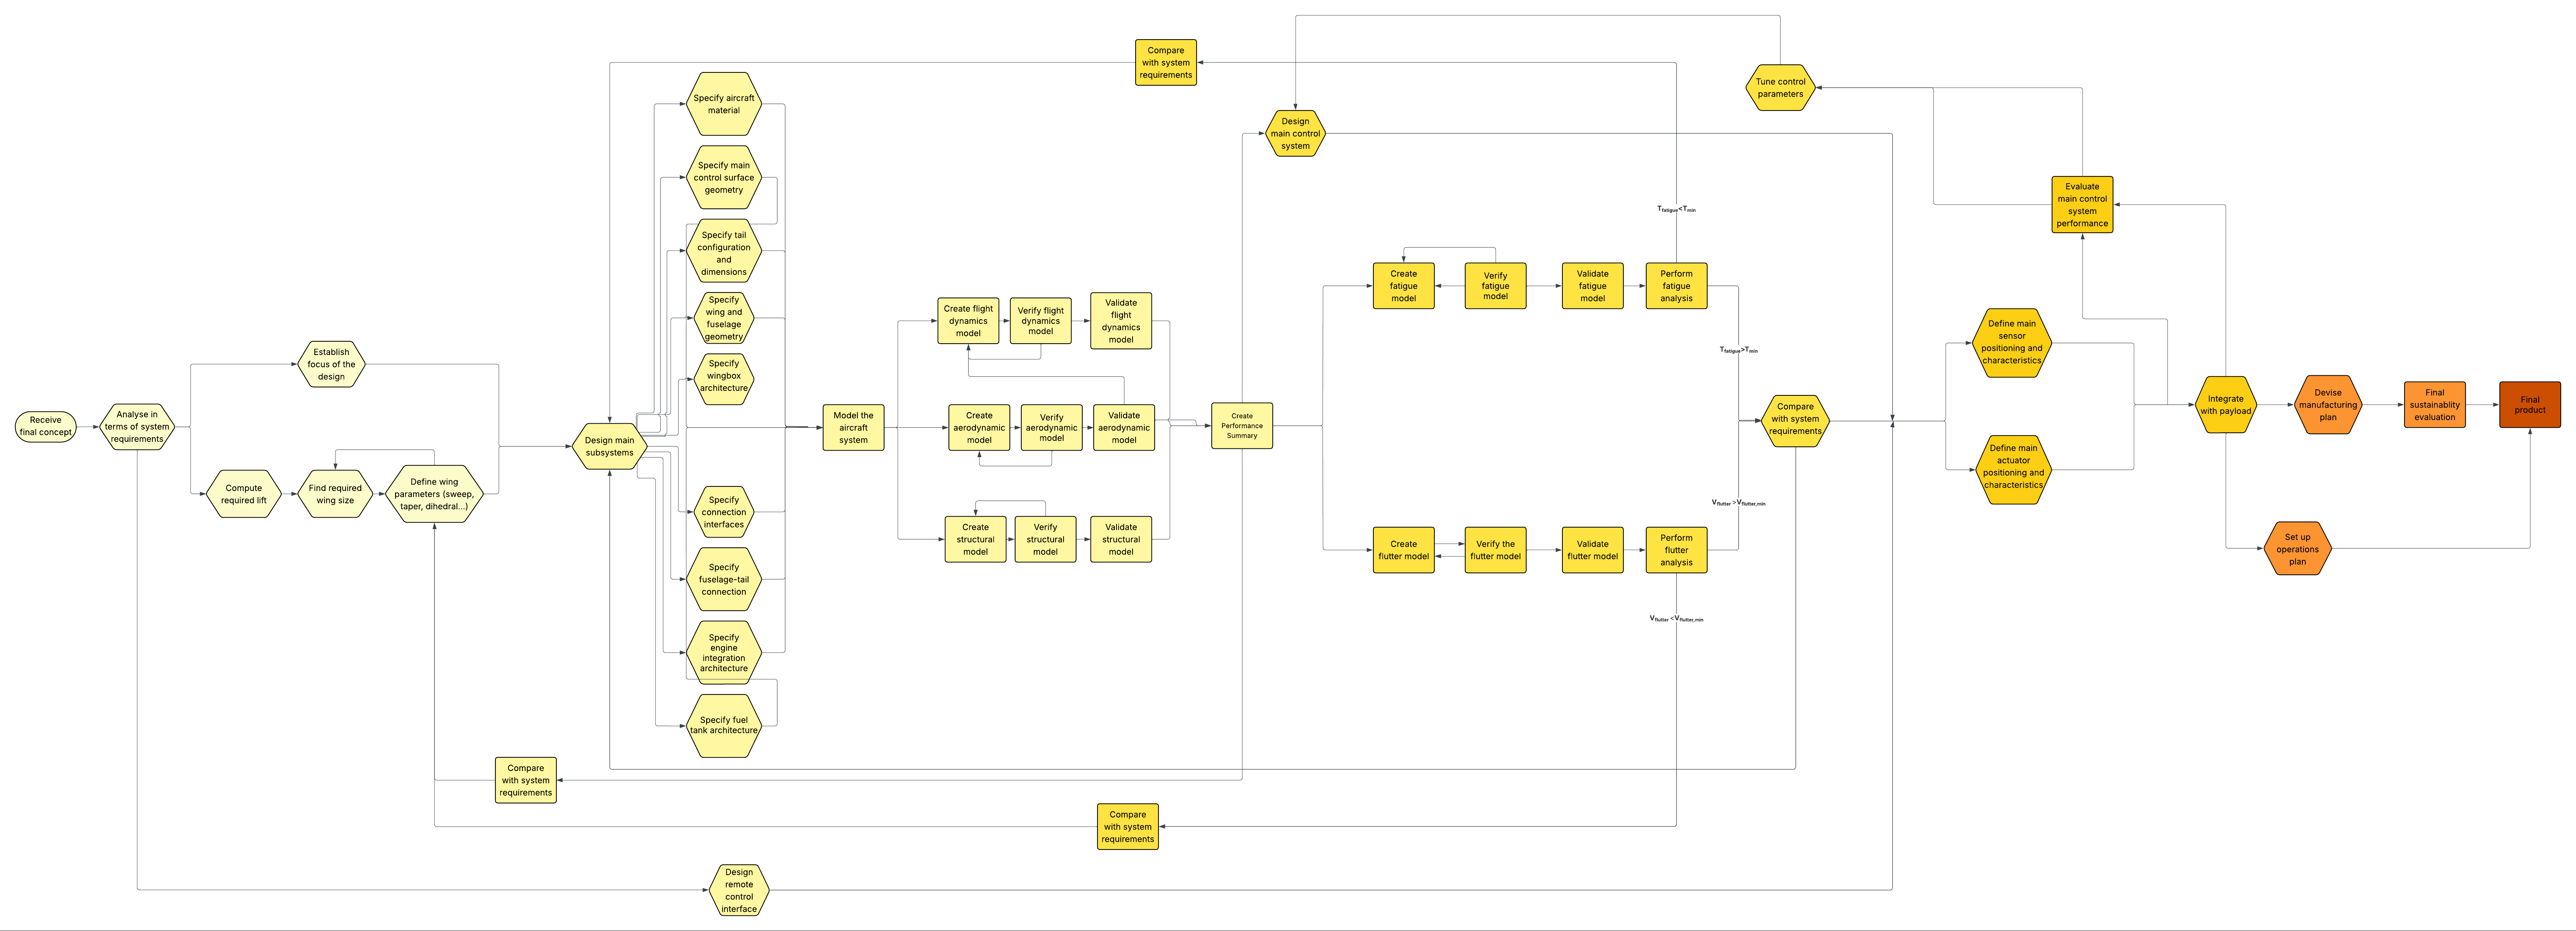
\includegraphics[width=1.1\linewidth]{figures/Final workflow.png}
%     \caption{Final Review Workflow Diagram}
%     \label{fig:workflow_final}
% \end{figure}


\section{Work Breakdown Structure}

A Work Breakdown Structure (WBS) is a hierarchical decomposition of a project into smaller, manageable components. It organizes all the work required to deliver a system into clearly defined elements, typically moving from high-level system functions down to detailed tasks or deliverables. The purpose of a WBS is to improve clarity, assign responsibility, support scheduling and budgeting, and ensure that no critical scope is overlooked.

In the case of the unmanned versatile test bed, two key aspects were considered when constructing the WBS: the physical system (air vehicle, payload, control), and the mission purpose (experimental testing, replacing conventional wind tunnels). This separation is important because, unlike a conventional aircraft project, the primary output is not the vehicle itself but the data and experimental capability it provides. Testing is elevated from a verification step to a core operational function. This reflects the idea that the platform acts as a “flying laboratory,” addressing limitations of wind tunnels such as mounting interference, scaling constraints, and inability to test to failure.

\begin{figure}[H]
    \centering
    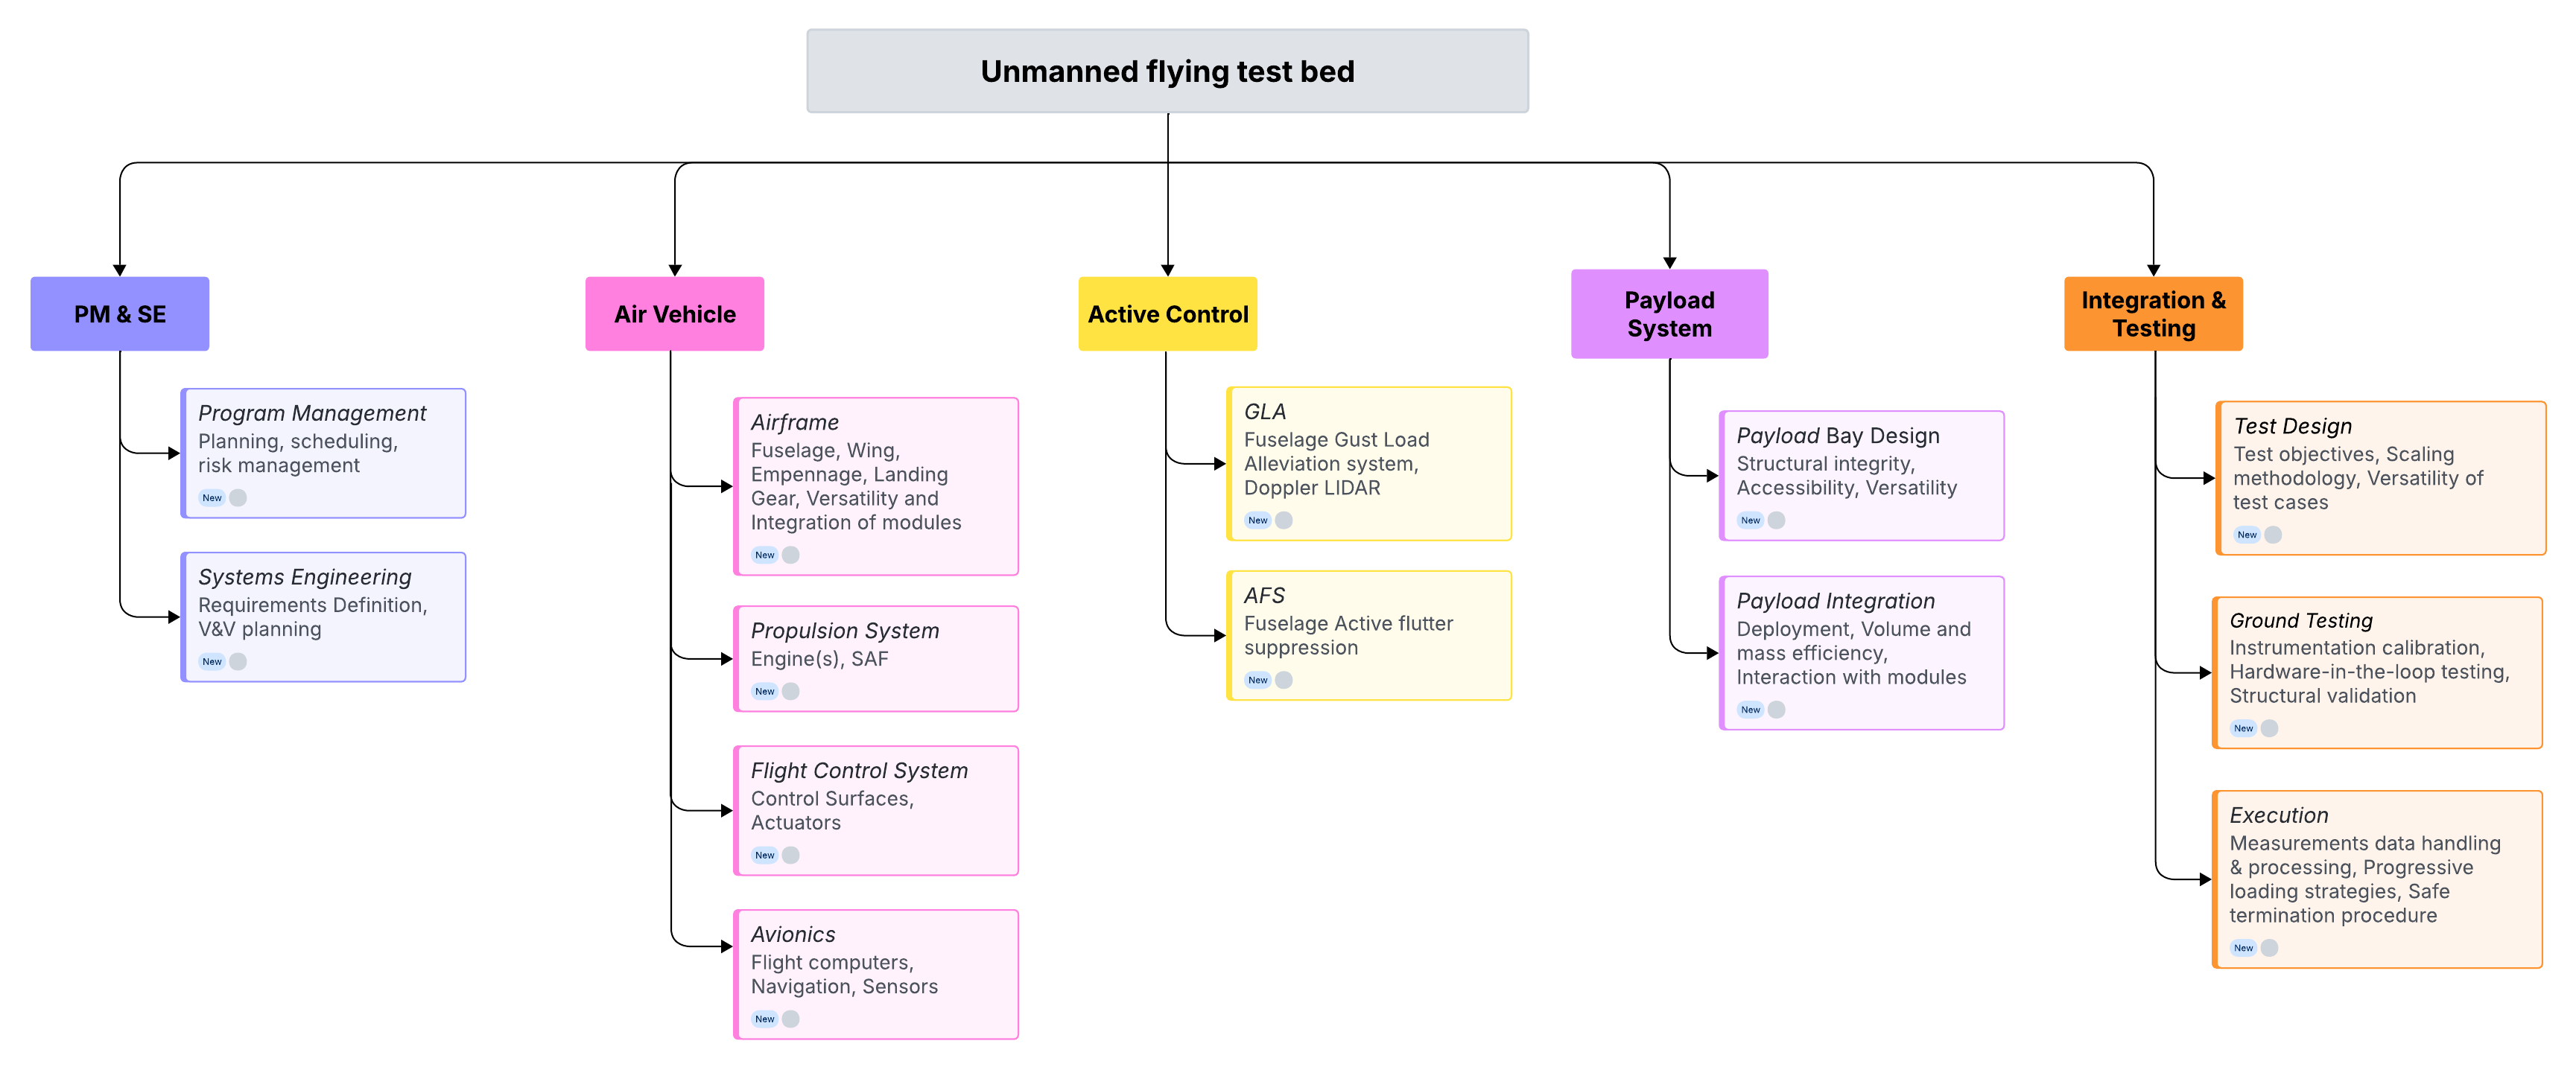
\includegraphics[width=1.1\linewidth]{figures/Work breakdown structure (WBS) (1).png}
    \caption{Work Breakdown Structure of the Unmanned Flying Laboratory}
    \label{fig:placeholder}
\end{figure}




\section{Schedule (Gantt Chart)}
To outline the schedule of the project, all the required deliverables and milestones have been compiled into a Gantt Chart, seen at the end of this chapter. It has been decided to work on the large reports: Project Plan, the Baseline Review, the Midterm Review and the Final Review in sequence, completing all other assignments, such as presentation preparation or posters, in parallel.

The three main reports of the project - the Baseline, Midterm and Final reports, are further subdivided into sub-tasks. This ensures that the team stays on schedule within the large work package. For contingency, all the sub-tasks are to be finished a full day before the day of the draft deadline. This is to avoid potentially low-quality last-minute corrections.

The tasks for the baseline report, whose goal is to create a broad overview of the design, can be efficiently parallelized, with extra time remaining for shortlisting of the configuration after other tasks are completed. The tasks of the midterm report, requiring the preparation and execution of a trade-off have to be completed in a more sequential matter. For the final report, the final sizing method and its verification and validation will be worked on simultaneously, following the paradigm of test-driven development.





\includepdf[pages=-,fitpaper=true, width=420mm, keepaspectratio]{figures/GantChart.pdf}